\documentclass[a4paper,14pt]{article}

\usepackage{comment} % Para comentar várias linhas ao mesmo tempo

%matemática
\usepackage{amsmath}
\usepackage{amssymb}

%diagramação
\usepackage{extsizes}
\everymath{\displaystyle}
\usepackage{geometry}
\usepackage{fancyhdr}
\usepackage{multicol}
\usepackage{graphicx}
\usepackage[brazil]{babel}
\usepackage[shortlabels]{enumitem}
\usepackage{cancel}
\usepackage{textcomp}
\usepackage{tcolorbox}

%tabelas
\usepackage{array} % Para melhor formatação de tabelas
\usepackage{longtable}
\usepackage{booktabs}  % Para linhas horizontais mais bonitas
\usepackage{float}   % Para usar o modificador [H]
\usepackage{caption} % Para usar legendas em tabelas
\usepackage{wrapfig} % Para usar tabelas e figuras flutuantes
\usepackage{xcolor} % Para cores do fundo de tabelas
\usepackage{colortbl} % Para cores do fundo de tabelas

%tikzpicture
\begin{comment}
	\usepackage{tikz}
	\usepackage{scalerel}
	\usepackage{pict2e}
	\usepackage{tkz-euclide}
	\usetikzlibrary{calc}
	\usetikzlibrary{patterns,arrows.meta}
	\usetikzlibrary{shadows}
	\usetikzlibrary{external}
\end{comment}


%pgfplots
\usepackage{pgfplots}
\pgfplotsset{compat=newest}
\usepgfplotslibrary{statistics}
\usepgfplotslibrary{fillbetween}

%colours
\usepackage{xcolor}



\columnsep=2cm
\hoffset=0cm
\textwidth=8cm
\setlength{\columnseprule}{.1pt}
\setlength{\columnsep}{2cm}
\renewcommand{\headrulewidth}{0pt}
\geometry{top=1in, bottom=1in, left=0.7in, right=0.5in}

\pagestyle{fancy}
\fancyhf{}
\fancyfoot[C]{\thepage}

\begin{document}
	
	\noindent\textbf{6FMA143 - Matemática} 
	
	\begin{center}Ampliações e reduções (Versão estudante)
	\end{center}
	
	\noindent\textbf{Nome:} \underline{\hspace{10cm}}
	\noindent\textbf{Data:} \underline{\hspace{4cm}}
	
	%\section*{Questões de Matemática}
	
	\begin{multicols}{2}
	    \noindent Figuras obtidas através de ampliações ou reduções são \textbf{sempre} semelhantes. \\
		\noindent\textsubscript{--------------------------------------------------------------------------}
		\begin{enumerate} 
			\item Uma máquina copiadora pode ter a função de ampliar ou reduzir cópias. O que significa isso? \\\\\\\\\\\\\\\\\\\\\\\\\\\\\\\\\\\\
			\item Carlos desenhou um triângulo em uma folha de seu fichário e usou uma fotocopiadora para fazer uma reprodução. A seguir são apresentados o desenho original de Carlos (primeira figura) e o triângulo da fotocópia, que Carlos recortou e colou em outra folha do fichário (segunda figura). \\
			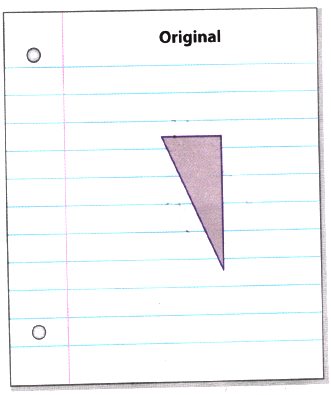
\includegraphics[width=1\linewidth]{6FMA143_imagens/imagem1}
			\\
			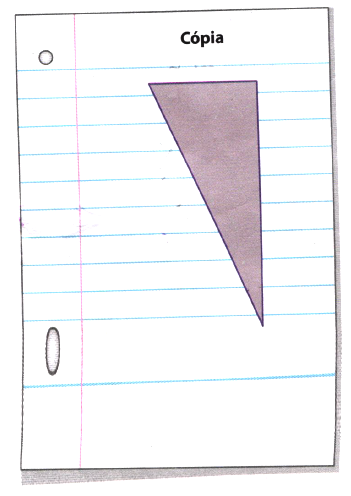
\includegraphics[width=1\linewidth]{6FMA143_imagens/imagem2}
			\newpage
			\begin{enumerate}[a)]
				\item Ele mandou fazer uma redução ou uma ampliação? \\\\\\\\\\
				\item De quantos por cento foi a variação do tamanho? \\\\\\\\\\
				\item A figura original e a cópia são congruentes ou semelhantes? \\\\\\\\\\
			\end{enumerate}
			\item O desenho abaixo mostra um triângulo, e logo a seguir sua ampliação. \\
			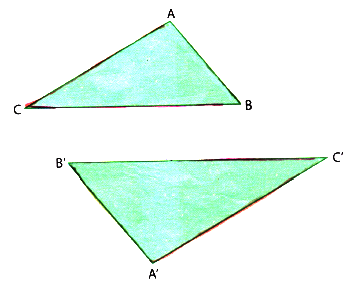
\includegraphics[width=1\linewidth]{6FMA143_imagens/imagem3}
			\begin{enumerate}[a)]
				\item Qual foi o percentual de ampliação? \\\\\\
				\item Meça, com muito cuidado, os ângulos internos triângulo $ABC$ e os do triângulo $A'B'C'$, completando a tabela a seguir:
				\renewcommand{\arraystretch}{2} % Aumenta o tamanho das linhas para o dobro
				\resizebox{6.5cm}{!}{
				\begin{tabular}{|c|c|c|c|}
					\hline
					$m(\hat{A})$ & ~~~~~~~~~ & $m(\hat{A}')$ & ~~~~~~~~~\\ \hline
					$m(\hat{B})$ & ~~~~~~~~~ & $m(\hat{B}')$ & ~~~~~~~~~\\ \hline
					$m(\hat{C})$ & ~~~~~~~~~ & $m(\hat{C}')$ & ~~~~~~~~~\\ \hline
				\end{tabular}
				}
				\\\\ Qual é a sua conclusão?  \\\\\\\\\\\\\\\\\\
				\item Meça, com precisão, os lados do triângulo $ABC$ e os do triângulo $A'B'C'$ e complete a tabela a seguir: \\
				\renewcommand{\arraystretch}{2} % Aumenta o tamanho das linhas para o dobro
				\resizebox{6.5cm}{!}{
				\begin{tabular}{|c|c|c|c|}
					\hline
					$AB$ & ~~~~~~~~~ & $A'B'$ & ~~~~~~~~~\\ \hline
					$AC$ & ~~~~~~~~~ & $A'C'$ & ~~~~~~~~~\\ \hline
					$BC$ & ~~~~~~~~~ & $B'C'$ & ~~~~~~~~~\\ \hline
				\end{tabular}
				}
				\\\\ Usando sua calculadora, obtenha os quocientes a seguir (se necessário, utilize uma aproximação com duas casas decimais após a vírgula):\\
				
				\renewcommand{\arraystretch}{3} % Aumenta o tamanho das linhas para o dobro
				
				\resizebox{6.5cm}{!}{
					\begin{tabular}{|c|c|c|c|}
						\hline
						$\frac{AB}{AC}$ & ~~~~~~~~~ & $\frac{A'B'}{A'C'}$ & ~~~~~~~~~\\ \hline
						$\frac{AB}{BC}$ & ~~~~~~~~~ & $\frac{A'B'}{B'C'}$ & ~~~~~~~~~\\ \hline
						$\frac{AC}{CC}$ & ~~~~~~~~~ & $\frac{A'C'}{B'C'}$ & ~~~~~~~~~\\ \hline
					\end{tabular}
				}
				\renewcommand{\arraystretch}{3} % Aumenta o tamanho das linhas para o dobro
				
				\resizebox{3.25cm}{!}{
					\begin{tabular}{|c|c|}
						\hline
						$\frac{AB}{A'B'}$ & ~~~~~~~~~ \\ \hline
						$\frac{AC}{A'C'}$ & ~~~~~~~~~ \\ \hline
						$\frac{BC}{B'C'}$ & ~~~~~~~~~ \\ \hline
					\end{tabular}
				}
				\\\\ Faça um relatório descrevendo e interpretando os resultados obtidos anteriormente. \\\\\\\\\\\\\\\\\\\\\\\\\\\\\\\\\\\\\\\\
			\end{enumerate}
			\item É dado o triângulo $ABC$ a seguir. Escolha, entre os triângulos apresentados no quadro seguinte, qual é uma redução do triângulo $ABC$. \\
			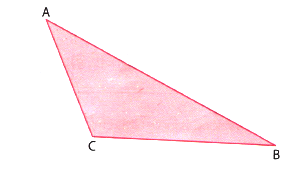
\includegraphics[width=1\linewidth]{6FMA143_imagens/imagem4}
			\\
			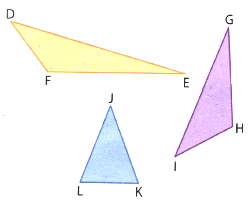
\includegraphics[width=1\linewidth]{6FMA143_imagens/imagem5}
			\newpage
			%79 a 82
			\item Observe os retângulos na malha quadriculada abaixo (cada quadrado tem 1 cm² de área):
			\\
			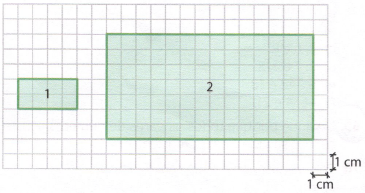
\includegraphics[width=1\linewidth]{6FMA143_imagens/imagem6}
			\begin{enumerate}[a)]
				\item Qual é a porcentagem de ampliação? \\\\\\\\\\\\\\\\
				\item Qual é o perímetro do retângulo 1? E do retângulo 2? A porcentagem de ampliação do perímetro é igual à porcentagem de ampliação dos lados dos retângulos? Justifique. \\\\\\\\\\\\\\\\
				\item Qual é a área do retângulo 1? E do retângulo 2? A porcentagem de ampliação da área é igual à porcentagem de ampliação dos lados dos retângulos? Justifique. \\\\\\\\\\\\\\\\
			\end{enumerate}
			\item O triângulo da direita é uma ampliação de 100\% do $\Delta$$ABC$. \\
			\\
			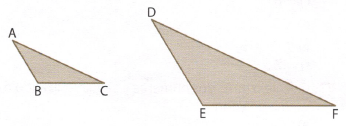
\includegraphics[width=1\linewidth]{6FMA143_imagens/imagem7} \\
			Sabendo que $AB = 4, AC = 8$ e $BC = 7$, determine $DE, DF$ e $EF$. \newpage
			\item No $\Delta$$ABC, AB = 5, AC = 9$ e $BC = 12$. No $\Delta$$DEF, DE = 2,4, EF = 1$ e $DF = 1,8$.
			\begin{enumerate}[a)]
				\item Complete: $\Delta$$ABC \thicksim \Delta ........ .$ \\\\\\\\\\\\\\\\\\\\
				\item $m (\hat{A}) = m(.....); m (\hat{B}) = m (.....); m (\hat{C}) = m (.....)$. \\\\\\\\\\\\\\\\\\\\
				\item O triângulo $ABC$ é uma ampliação ou uma redução do triângulo $DEF$? \\\\\\\\\\\\\\\\\\\\\\
			\end{enumerate}
			\item Os paralelepípedos a seguir são semelhantes. Determine a porcentagem de ampliação.
			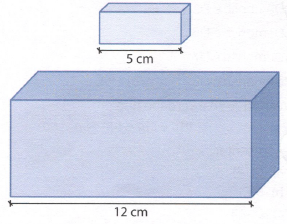
\includegraphics[width=1\linewidth]{6FMA143_imagens/imagem8}
		\end{enumerate}
		$~$ \\ $~$ \\ $~$ \\ $~$ \\ $~$ \\ $~$ \\ $~$ \\ $~$ \\ $~$ \\ $~$ \\ $~$ \\ $~$ \\ $~$ \\ $~$ \\ $~$ \\ $~$ \\ $~$ \\ $~$ \\ $~$ \\ $~$ \\ $~$ \\ $~$ \\ $~$ \\ $~$ \\ $~$ \\ $~$ \\ $~$ \\ $~$ \\ 
	\end{multicols}
\end{document}